\chapter{Execution}
    \section{Calibration of the Force Sensor} \label{sec:Calibration}
        First, the measurement setup must be calibrated. For this purpose, three calibration weights are selected from a choice
        of weights. These are first weighed on the balance provided in the laboratory. They are then hung on the cantilever with
        the strain gauges in alternating arrangements, i.e. alone and in various combinations. The \textsc{Du Noüy}-ring, which
        is required for later measurements, is removed in the meantime. Care is taken to ensure that the weights do not swing.
        For each arrangement, the offset button is first pressed and the data recorded for about \(30\) seconds and stored in a text
        file.
        %
    \section{Resolution and Statistics} \label{sec:Statistics}
        The variance of the conversion result is analyzed by repeating the procedure from \cref{sec:Calibration}, but without
        additional weights. The values are recorded and stored over a period of \SI{100}{s}.
        %
    \section{Measurement of Surface Tension} \label{sec:Surface_Tension}
        To avoid unnecessary errors when measuring the surface tension due to impurities, the \textsc{Du Noüy}-ring is first washed with tap
        water and subsequently rinsed with distilled water. A paper towel is used for drying and any skin contact is avoided
        not to re-contaminate the surface of the ring. After the cleaning, it is carefully hung in the hook on the boom.\par
        \begin{figure}[h]
		    \centering
		    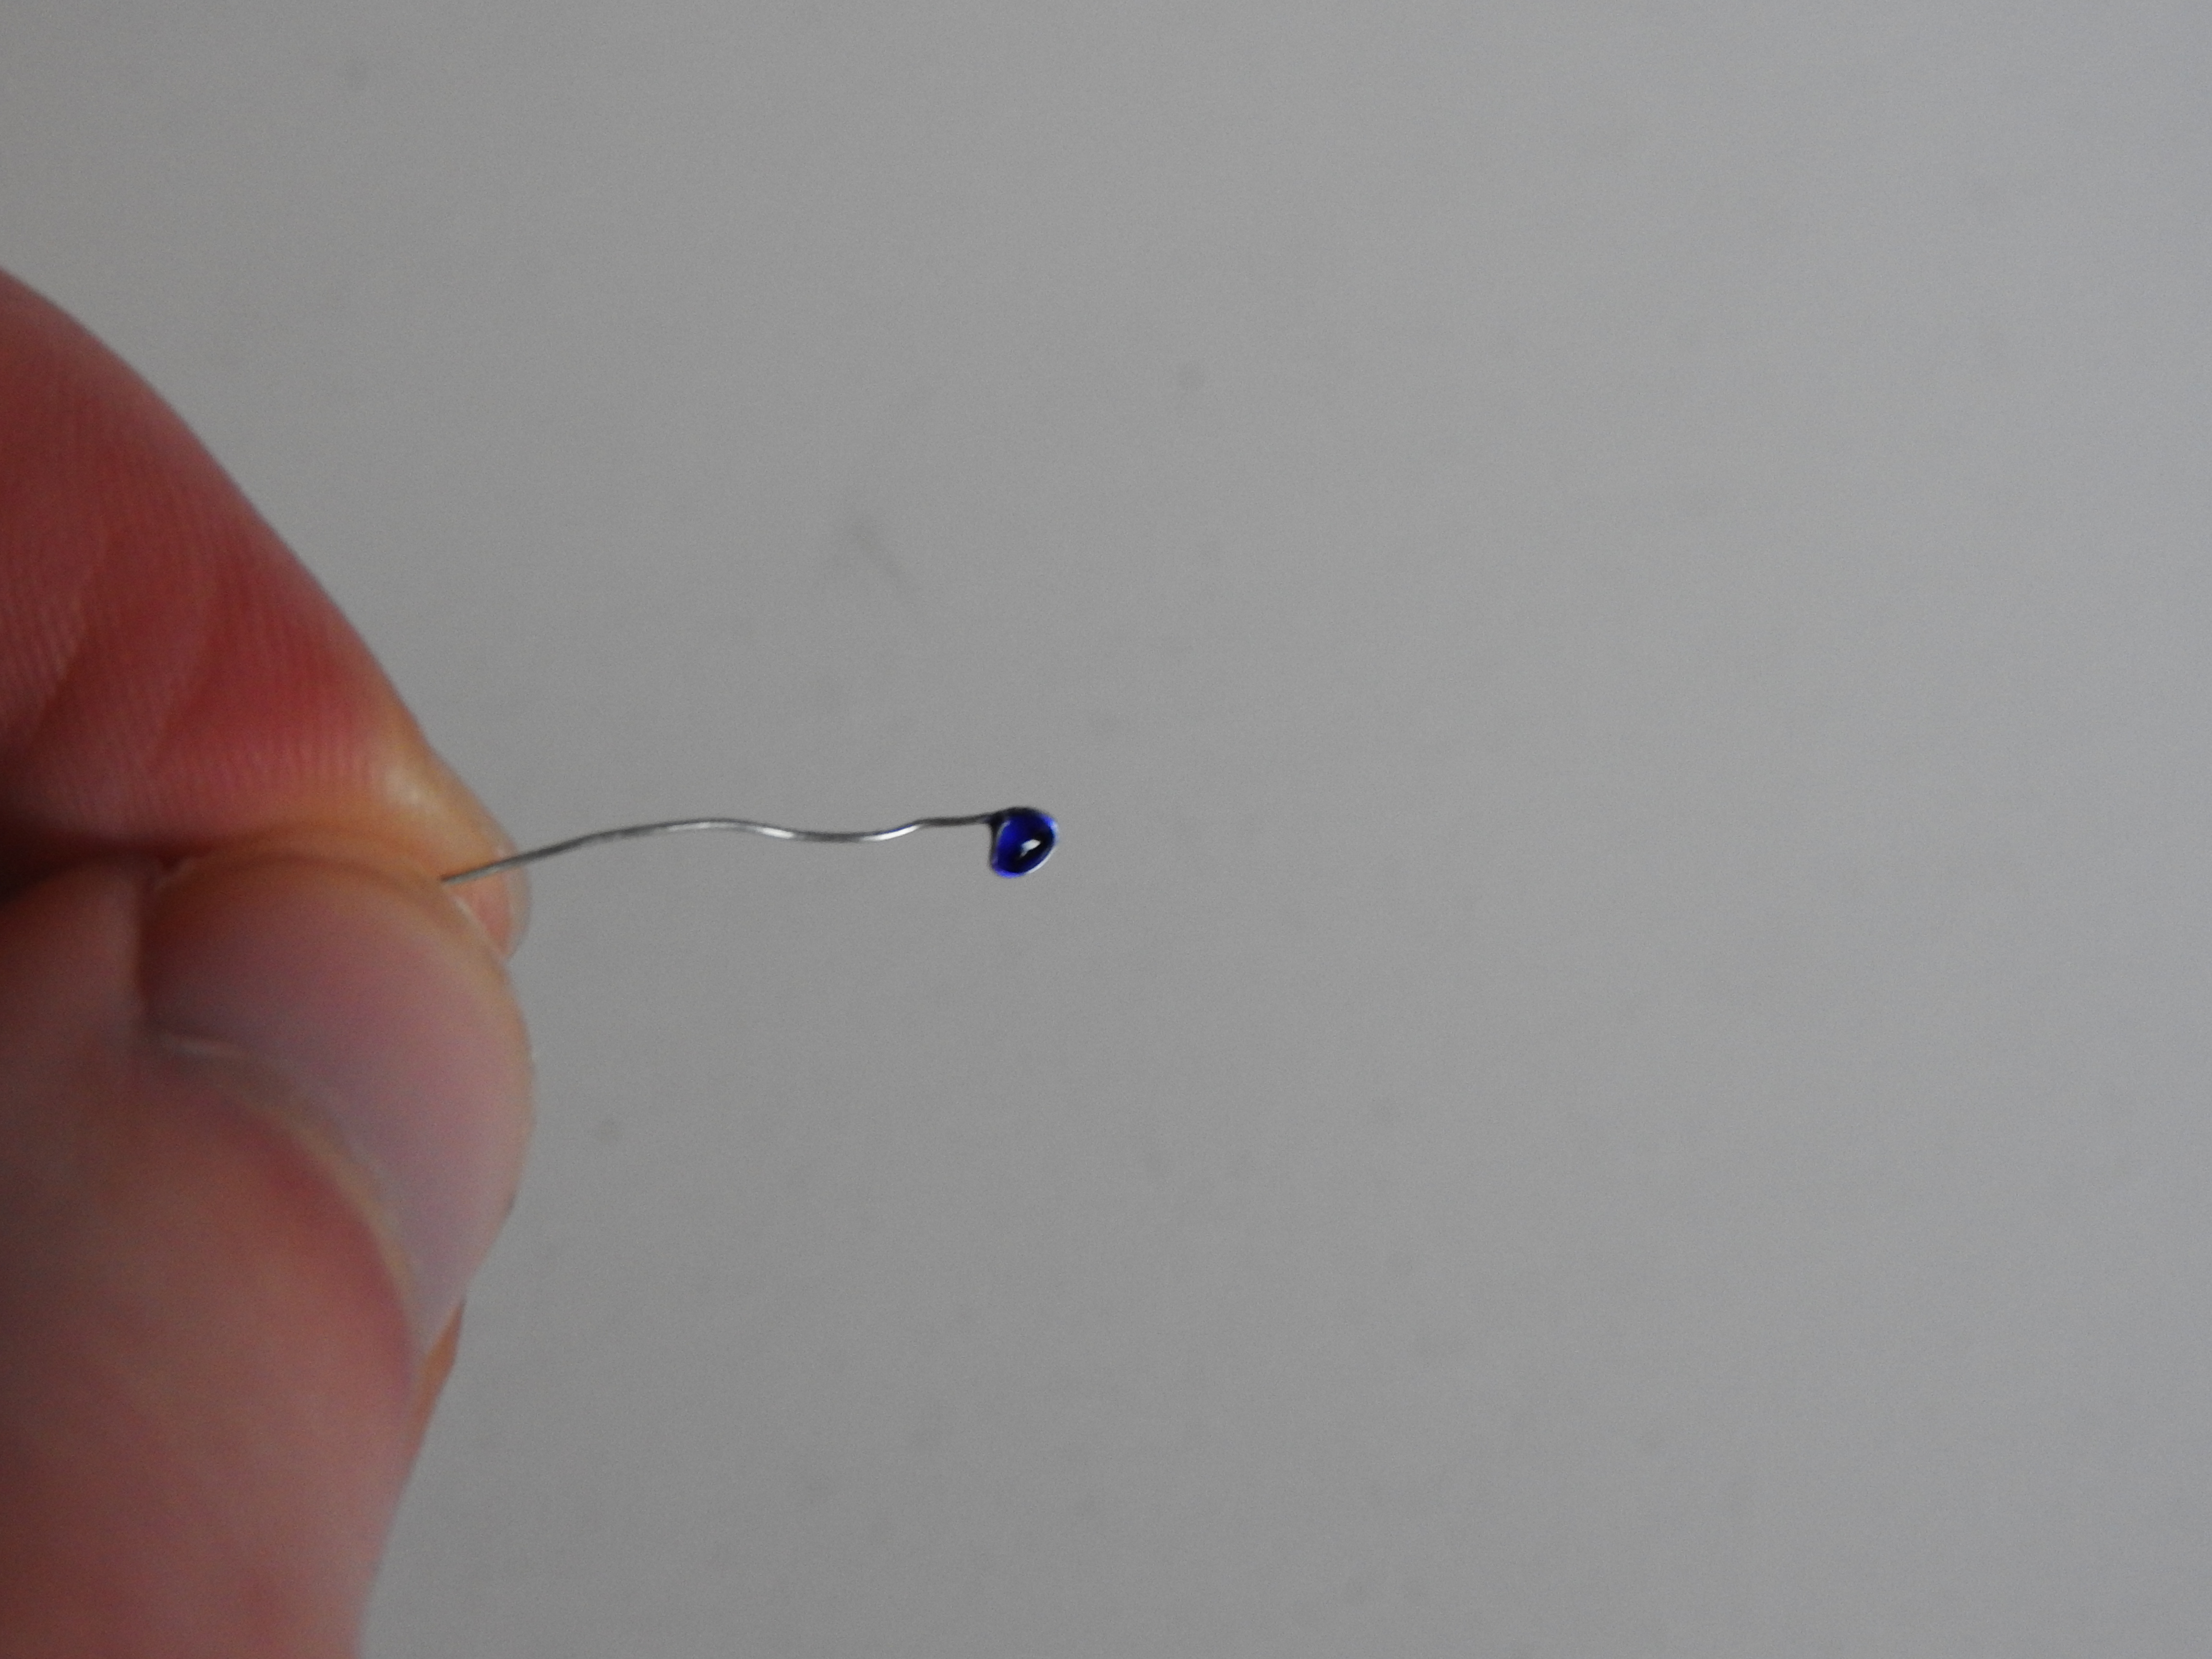
\includegraphics[width=.6\textwidth]{aufbau/wire_detergent.jpg}
		    \caption[Method of dosing detergent]{Method of dosing detergent. The tip of a thin wire is dipped in detergent to transfer a small amount to the distilled water containing beaker.}
		    \label{fig:wire_detergent}
	    \end{figure}
        A glass beaker is filled with distilled water to the point where the ring can be
        completely immersed. The beaker is placed on a height-adjustable platform just below the ring. The ring is now aligned as
        parallel as possible to the water surface. To stabilize the alignment of the ring, a piece of thin wire is also wrapped
        around the holding strings. Now the platform is turned upwards until the ring almost touches the water. The offset button
        is pressed and the recording of the values is started with \textsc{RealTerm}. Now the platform is slowly moved further up
        until the ring is completely covered with water. Then the platform is lowered again until the ring is no longer in contact
        with the water and the lamella is torn. The data is stored. This procedure is repeated until 10 measurements have been
        recorded. After the measurement with pure water has been completed, the behavior is examined when detergent is dissolved
        in the water. To do this, the tip of a thin wire is bend to a little circle which can hold a small amount of detergent
        after dipping the tip into it (\cref{fig:wire_detergent}). After that the tip is immersed into the water and stirred until the detergent is fully
        solved. Again, 10 series of measurements are recorded according to the same scheme. Then a second time detergent is stirred
        in with the tip of the wire and again 10 measurements are recorded. Finally, the water is tipped away and the beaker is
        filled with 2-isopropanol. Again, 10 measurements are recorded according to the same scheme. Finally, the diameter of the
        ring is measured with a caliper.
        %